% !TeX root = 00P1_cae_ontology.tex

\clearpage
\section*{Appendix D. Diagrammatic Intuition}
\addcontentsline{toc}{section}{Appendix D. Diagrammatic Intuition}

This appendix provides informal diagrams for the entity kinds, relationships,
and accountability chains introduced in the main text.
The goal is to support intuition rather than to introduce new formal content.

% ------------------------------------------------------------
\subsection*{D.1 Entity Kinds and Disjointness}
% ------------------------------------------------------------

Figure~\ref{fig:entity-kinds} depicts the six entity kinds as disjoint sets.

\begin{figure}[ht]
    \centering
    \begin{tikzpicture}[
            kind/.style={ellipse,draw,minimum width=2.5cm,minimum height=1.5cm,align=center},
            node distance=1.2cm
        ]
        % Top row
        \node[kind,fill=blue!10] (A) {Actors\\(A)};
        \node[kind,fill=green!10,right=of A] (S) {Sites/Assets\\(S)};
        \node[kind,fill=orange!10,right=of S] (I) {Instruments\\(I)};

        % Bottom row
        \node[kind,fill=red!10,below=of A] (E) {Events\\(E)};
        \node[kind,fill=purple!10,below=of S] (J) {Jurisdictions\\(J)};
        \node[kind,fill=yellow!10,below=of I] (O) {Observations\\(O)};
    \end{tikzpicture}
    \caption{The six disjoint entity kinds in CAE. Each entity belongs to exactly
        one kind, and kinds do not overlap.}
    \label{fig:entity-kinds}
\end{figure}


% ------------------------------------------------------------
\subsection*{D.2 Accountability Chain: Statute to Outcomes}
% ------------------------------------------------------------


Figure~\ref{fig:accountability-chain} visualizes an accountability chain from
a federal statute through regulatory implementation to observed outcomes.

\begin{figure}[ht]
    \centering
    \begin{tikzpicture}[
            node distance=2.5cm,
            actor/.style={rectangle,rounded corners,draw,fill=blue!10,minimum width=2.2cm,minimum height=0.9cm,align=center},
            inst/.style={rectangle,rounded corners,draw,fill=orange!10,minimum width=2.2cm,minimum height=0.9cm,align=center},
            event/.style={rectangle,rounded corners,draw,fill=red!10,minimum width=2.2cm,minimum height=0.9cm,align=center},
            obs/.style={rectangle,rounded corners,draw,fill=yellow!10,minimum width=2.2cm,minimum height=0.9cm,align=center},
            >=Latex
        ]
        % Top: Actors
        \node[actor] (congress) {Congress\\(Actor)};
        \node[actor,right=of congress] (agency) {Agency\\(Actor)};

        % Middle: Instruments
        \node[inst,below=1.5cm of congress] (statute) {Statute\\(Instrument)};
        \node[inst,below=1.5cm of agency] (reg) {Regulation\\(Instrument)};
        \node[inst,right=of reg] (permit) {Permit\\(Instrument)};

        % Bottom: Events
        \node[event,below=1.5cm of reg] (payment) {Payment\\(Event)};
        \node[event,right=of payment] (inspection) {Inspection\\(Event)};

        % Outcomes
        \node[obs,below=1.5cm of payment] (outcome) {Health Outcome\\(Observation)};

        % Relationships
        \draw[->] (congress) -- node[left,font=\small] {enacts} (statute);
        \draw[->] (agency) -- node[right,font=\small] {issues} (reg);
        \draw[->] (statute) -- node[above,font=\small] {implements} (reg);
        \draw[->] (reg) -- node[above,font=\small] {authorizes} (permit);
        \draw[->] (permit) -- node[left,font=\small] {occurs-under} (payment);
        \draw[->] (permit) -- node[right,font=\small] {occurs-under} (inspection);
        \draw[->] (payment) -- node[left,font=\small] {associated-with} (outcome);
        \draw[->] (inspection) -- node[right,font=\small] {associated-with} (outcome);
    \end{tikzpicture}
    \caption{An accountability chain from normative instrument (statute) through
        regulatory implementation to observed outcomes. Authority flows downward,
        while Observations connect back to Events and Instruments.}
    \label{fig:accountability-chain}
\end{figure}

% ------------------------------------------------------------
\subsection*{D.3 Relationship Constraints by Entity Kind}
% ------------------------------------------------------------

Figure~\ref{fig:relationship-constraints} shows representative relationship
types and the entity kinds they connect.

\begin{figure}[ht]
    \centering
    \begin{tikzpicture}[
            node distance=3.5cm,
            kind/.style={circle,draw,minimum size=1.4cm,align=center,font=\small},
            >=Latex
        ]
        \node[kind,fill=blue!10] (A) {Actor\\(A)};
        \node[kind,fill=orange!10,right=of A] (I) {Instrument\\(I)};
        \node[kind,fill=red!10,below=of A] (E) {Event\\(E)};
        \node[kind,fill=green!10,below=of I] (S) {Site\\(S)};
        \node[kind,fill=purple!10,right=of I] (J) {Jurisdiction\\(J)};

        \draw[->] (A) -- node[above,font=\scriptsize] {enacts} (I);
        \draw[->] (A) -- node[left,font=\scriptsize] {party-to} (I);
        \draw[->] (I) -- node[right,font=\scriptsize] {occurs-under} (E);
        \draw[->] (E) -- node[below,font=\scriptsize] {involves} (A);
        \draw[->] (E) -- node[above,font=\scriptsize] {acts-on} (S);
        \draw[->] (S) -- node[right,font=\scriptsize] {located-in} (J);
        \draw[->] (I) -- node[above,font=\scriptsize] {applies-in} (J);
    \end{tikzpicture}
    \caption{Representative relationship types constrained by source and target
        entity kinds. For example, \emph{enacts} requires Actor $\rightarrow$ Instrument.}
    \label{fig:relationship-constraints}
\end{figure}

% ------------------------------------------------------------
\subsection*{D.4 Role Emergence from Relationship Patterns}
% ------------------------------------------------------------

Figure~\ref{fig:role-patterns} illustrates how a university (single Actor)
occupies multiple roles through different relationship patterns.

\begin{figure}[ht]
    \centering
    \begin{tikzpicture}[
            node distance=2.8cm,
            actor/.style={ellipse,draw,fill=blue!10,minimum width=2.2cm,minimum height=1.2cm,align=center},
            other/.style={rectangle,rounded corners,draw,minimum width=2.0cm,minimum height=0.9cm,align=center},
            >=Latex
        ]
        % Central actor
        \node[actor] (U) {University\\(Actor)};

        % Related entities
        \node[other,fill=orange!10,above left=1.8cm and 2.5cm of U] (grant) {NSF Grant\\(Instrument)};
        \node[other,fill=green!10,above right=1.8cm and 2.5cm of U] (lab) {Lab\\(Site)};
        \node[other,fill=red!10,below=of U] (inspection) {Inspection\\(Event)};

        % Relationships showing different roles
        \draw[->] (grant) -- node[above left,font=\scriptsize,align=center] {party-to \\ (recipient)} (U);
        \draw[->] (U) -- node[above right,font=\scriptsize,align=center] {operates \\ (operator)} (lab);
        \draw[->] (inspection) -- node[right,font=\scriptsize,align=center] {subject-of \\ (regulated)} (U);
    \end{tikzpicture}
    \caption{A single Actor (university) occupies multiple roles (recipient,
        operator, regulated entity) through different relationship patterns.
        Roles emerge from structure, not from entity kind.}
    \label{fig:role-patterns}
\end{figure}

% ------------------------------------------------------------
\subsection*{D.5 Temporal Structure: Enduring vs Time-Indexed Entities}
% ------------------------------------------------------------

Figure~\ref{fig:temporal-structure} contrasts enduring entities (Actors,
Instruments, Sites, Jurisdictions) with time-indexed entities (Events, Observations).

\begin{figure}[ht]
    \centering
    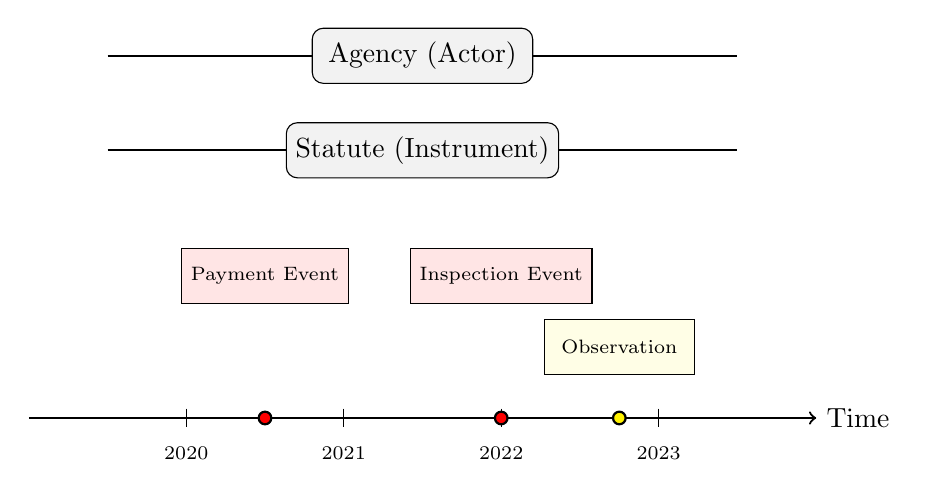
\begin{tikzpicture}[
            enduring/.style={rectangle,rounded corners,draw,fill=gray!10,
                    minimum width=2.8cm,minimum height=0.7cm,align=center},
            temporal/.style={rectangle,draw,fill=red!10,
                    minimum width=1.9cm,minimum height=0.7cm,align=center},
            obs/.style={rectangle,draw,fill=yellow!10,
                    minimum width=1.9cm,minimum height=0.7cm,align=center},
        ]

        % Timeline
        \draw[thick,->] (0,0) -- (10,0) node[right] {Time};
        \foreach \x in {2,4,6,8} {
                \draw (\x,0.12) -- (\x,-0.12);
            }
        \node at (2,-0.45) {\scriptsize 2020};
        \node at (4,-0.45) {\scriptsize 2021};
        \node at (6,-0.45) {\scriptsize 2022};
        \node at (8,-0.45) {\scriptsize 2023};

        % Enduring entity: Agency
        \draw[thick] (1,4.6) -- (9,4.6);      % draw line first
        \node[enduring] at (5,4.6) {Agency (Actor)};  % box on top

        % Enduring entity: Statute
        \draw[thick] (1,3.4) -- (9,3.4);
        \node[enduring] at (5,3.4) {Statute (Instrument)};

        % Events
        \draw[thick,fill=red] (3,0) circle (0.08);
        \node[temporal] at (3,1.8) {\scriptsize Payment Event};

        \draw[thick,fill=red] (6,0) circle (0.08);
        \node[temporal] at (6,1.8) {\scriptsize Inspection Event};

        % Observation
        \draw[thick,fill=yellow] (7.5,0) circle (0.08);
        \node[obs] at (7.5,0.9) {\scriptsize Observation};

    \end{tikzpicture}
    \caption{Temporal structure in CAE. Actors and Instruments are enduring
        entities that persist over time. Events and Observations are time-indexed
        occurrences.}
    \label{fig:temporal-structure}
\end{figure}
